\documentclass[11pt]{article}
\usepackage[utf8]{inputenc}
\usepackage{graphicx}
\graphicspath{ {./images/} }
\usepackage{graphics}
\usepackage{booktabs}
\usepackage{lipsum}
\usepackage{caption}
\usepackage{subcaption}
\usepackage[a4paper,width=150mm,top=30mm,bottom=30mm]{geometry}
%\usepackage{minted}
\usepackage{hyperref}
\usepackage{fancyhdr}
\usepackage{float}
\pagestyle{fancy}
\fancyhead{}
%\fancyhead[R]{Text}    % add text as header
\fancyfoot{}
\fancyfoot[C]{\thepage}   % add page number
\renewcommand{\headrulewidth}{0.10pt}
\renewcommand{\footrulewidth}{0.10pt}
\usepackage{listings}

\usepackage[
backend=biber, 
style=numeric,
sorting=none
]{biblatex}
\addbibresource{references.bib}

\usepackage{minted} % First pip install pygments

\setminted[python]{breaklines, framesep=2mm, fontsize=\footnotesize, numbersep=5pt}

%% \pagestyle{empty} remove header and footer for that page
%% \pagestyle{plain} add only the page number



\begin{document}



\begin{titlepage}
    \begin{center}
        \vspace*{1cm}
        
        \Huge
        \textbf{Antibody Sequence Analysis}

        \vspace{0.3cm}

        \rule{\textwidth}{.4pt}

        \vspace{0.5cm}
        
        \LARGE
        Sequence Logos from Multiple Sequence Alignment, Humanization Models 
        
        \vspace{5mm}
        
        \large
        \textbf{Enrico Frigoli, Lotte Draijer, Clara Canavese, Charlotte Resch}
         \vfill
        %\vspace{5mm}
        \begin{figure}[h]
		
\includegraphics[width=6cm]{sdu_logo_complete.png}
		\centering
	\end{figure}
  
        
        \vspace{10mm}
	\large
	Introduction to Bioinformatics  \\
	Prof. Konrad Krawczyk \\
	Fall 2022
        
        \vspace{5mm}
            
        Github: \href{https://github.com/enricofrigoli/bioinformatics\_fall22.git}{https://github.com/enricofrigoli/bioinformatics\_fall22.git}
        
		
        
        %\begin{center}
        %	
\includegraphics[width=0.4\textwidth]{sdu_logo_complete.png}
        %\end{center}
    
        

		
        
    \end{center}

\end{titlepage}

%\twocolumn[
%  \begin{@twocolumnfalse}
%    \begin{abstract}
%        \centering
%        Cancer genomics is the coolest thing in the world.
%    \end{abstract}
%  \end{@twocolumnfalse}
%]

% \parencite{}

%\vspace*{1cm}

\tableofcontents
\clearpage


\section{Introduction}

Antibodies are proteins produced by the immune system to respond to the presence of foreign substances. Antibodies are able to recognize unique parts on such substances, called antigens, and bind to those. %A lot of substances that enter the body are recognized as antigens by the antibodies, because the molecules on the surface of the invader are different from the molecules found in the body. Each antibody is identical to the antigen receptor of the B-cell, a type of white blood cell, that produced it. \newline

The basic structure of an antibody in mammals consists of two pairs of polypeptide chains that form a Y-shape \cite{encyclopedia}. The polypeptide chains can be distinguished in two identical heavy chains and two identical light chains, connected by disulfide bonds. Each chain is composed by a series of domains, that can be variable (V) or constant (C). 
The sub-region, called \textit{$F_V$}, that binds to the antigen is composed of the variable domain of the heavy chain and the variable domain of the light chain \cite{immunobiology}.

Each variable domain is usually subdivided into four Framework Regions (FRs) separated by three Complementary Determining Regions (CDRs), also called hypervariable regions. When the protein folds, the three CDRs come together on the surface of the antibody and create an antigen-binding site (together with the 3 CDRs of the other chain).

Thus, CDRs  differ significantly from antibody to antibody, since they are responsible for the affinity towards only one specific epitope, which is a distinct section of the antigen surface that is recognized by a specific antibody (different antibodies can recognized different epitopes of one antigen). 
Instead, the FRs serve as scaffold to hold the CDRs in position, thus they are expected to be more conserved across the range of all antibodies of a given species.

%Each of these two variable domains contains three hypervariable loops, known as Complementary Determining Regions (CDRs) distributed between the framework regions. It is the CDR regions that contain the recognition of the antigen. The high variability of these CDRs give the antibodies the ability to recognize an almost unlimited number of antigens \cite{MOREA2000267}. \newline
%\indent The Fc (fragment crystallizable) region is the tail region of the antibody that will interact with the cell surface receptors. Because of this, the immune system will be activated. These Fc regions have a highly conserved N-glycosylation site \cite{immunobiology}. \newline

In the development of therapeutic monoclonal antibodies, the starting point is often an immunized non-human organism, i.e. a mouse, which antibodies are collected and engineered to make them "more human", thus lowering the probability of having an anti-mouse response following administration. 

In this project, we explore the sequence variability of antibodies and the use of different tools to distinguish between mouse and human antibodies, in order to aid the humanization effort. The full code is available in the GitHub repository.



\section{Sequence Logos from Multiple Sequence Alignment}

The input files of our analysis are two FASTA files containing 9997 protein sequences each, representing the variable domain of the heavy chain of human and mouse antibodies respectively.

Thanks to the regular subdivision into CDRs and FRs of the sequences taken into consideration, it is possible to perform Multiple Sequence Alignment (MSA) to spot FRs segments and CDRs in the given sequences by looking at the variability of amino acid residues, given that FRs are expected to align together.


\subsection{Multiple Sequence Alignment}

To perform MSA we used both Clustal Omega \cite{clustal} and MUSCLE \cite{muscle}.
We downloaded Clustal Omega locally using \verb|conda| and ran it with the Biopython wrapper.
MUSCLE was also used locally by downloading the executable file and running the alignment via command line. We used the Super5 algorithm (\verb|-super5| argument) that allows to align large datasets more efficiently.


\subsection{Sequence Logo}

In sequence logos, the overall height of the stack indicates the \textit{information content} of the column, i.e., its relative entropy distance from an assumed background distribution, which measures the conservation of a position in a profile. % in a profile?
The height of symbols within the stack indicates the relative frequency of each amino acid at that position.

We used the output files from the MSA to generate the sequence logos. We installed WebLogo using \verb|pip|, then we wrote a bash script that automatically creates the sequence logos from previously generated FASTA files. 

\indent In both human and mouse sequence logos (Figures \ref{fig:muscle_logo}, \ref{fig:clustalo_logo}), we can see more conserved regions alternating with more variable regions. The former corresponds to the framework: a higher level of self information means lower entropy and so more conserved positions; the latter corresponds to the CDRs, that are the most variable parts of antibodies where the entropy is higher and positions are less conserved. As expected, there are 3 non-consecutive CDRs regions in both the human and the mouse variable region of the antibodies. 

\begin{figure}[h]
	
	\begin{subfigure}{0.5\textwidth}
		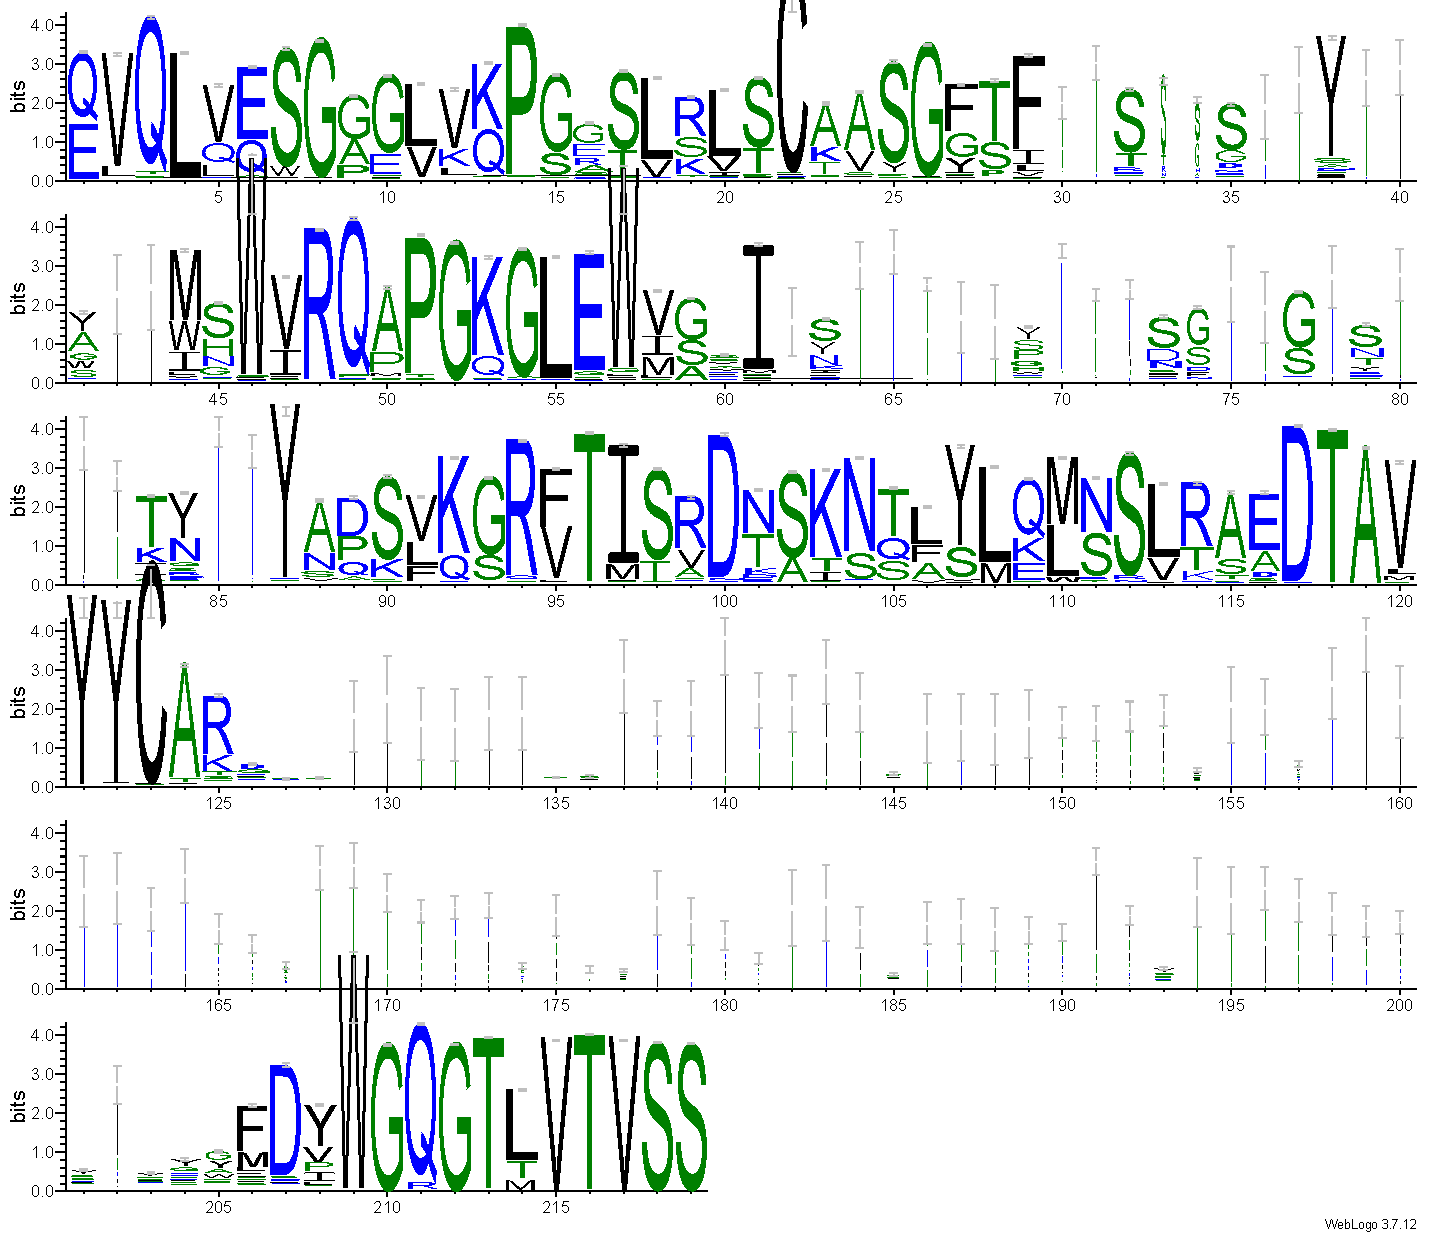
\includegraphics[width=0.9\linewidth, height=6cm]{images/human_msa_muscle_logo.pdf} 
		\caption{Human}
		%\label{fig:hlogo}
	\end{subfigure}
	\begin{subfigure}{0.5\textwidth}
		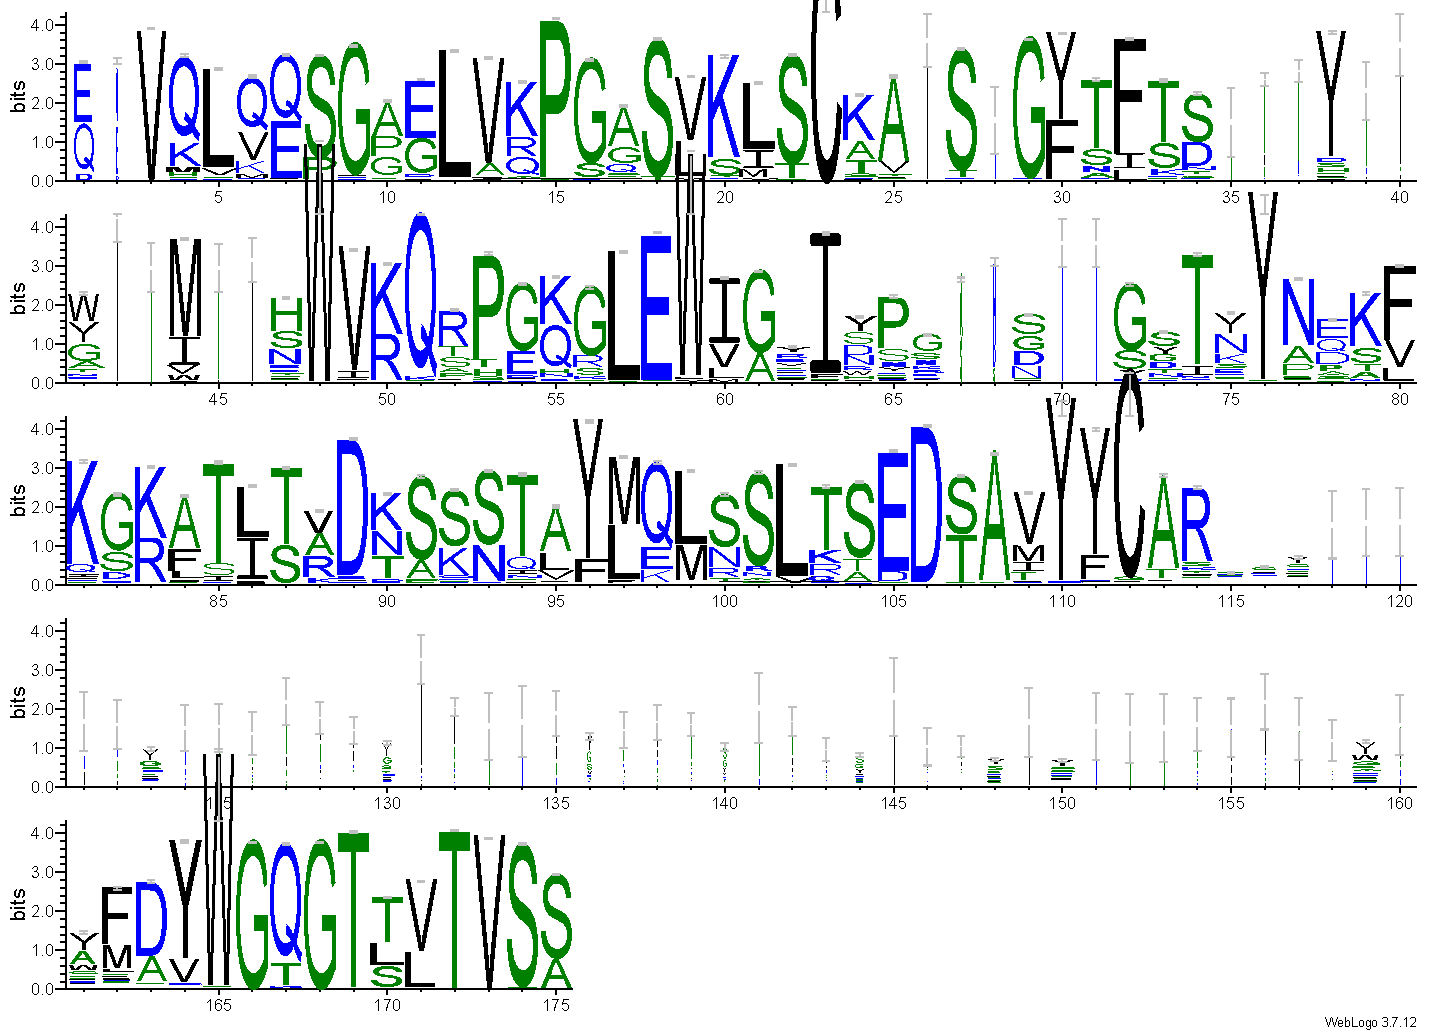
\includegraphics[width=0.9\linewidth, height=6cm]{images/mouse_msa_muscle_logo.pdf}
		\caption{Mouse}
		%\label{fig:mlogo}
	\end{subfigure}
	
	\caption{\small Sequence logos for human and mouse antibody sequences aligned with MUSCLE. The positions without letters are the result of a large percentage of gaps in a specific position across the MSA, thus, such positions should be ignored.}
	\label{fig:muscle_logo}
\end{figure}

\subsection{Antibody Numbering}

To perform \textit{antibody numbering} using the IMGT numbering scheme \cite{IMGT} we installed the ANARCI package \cite{anarci} via \verb|conda|. We used the \verb|run_anarci| wrapper to ensure parallel computation and direct FASTA parsing. The alignment was restricted to human or mouse germline only, depending on the dataset. After that, we created a Python function that takes the numbering CSV file as input and gives as output a FASTA file containing the aligned gapped sequences.
Finally, we created the Sequence Logos for both the human and the mouse sequences using WebLogo, as done in the previous section. In these logos (Figure \ref{fig:image2}), positions without letters correspond to positions in the alignment in which there is a high frequency of gaps. 

\begin{figure}[h]
	
	\begin{subfigure}{0.5\textwidth}
		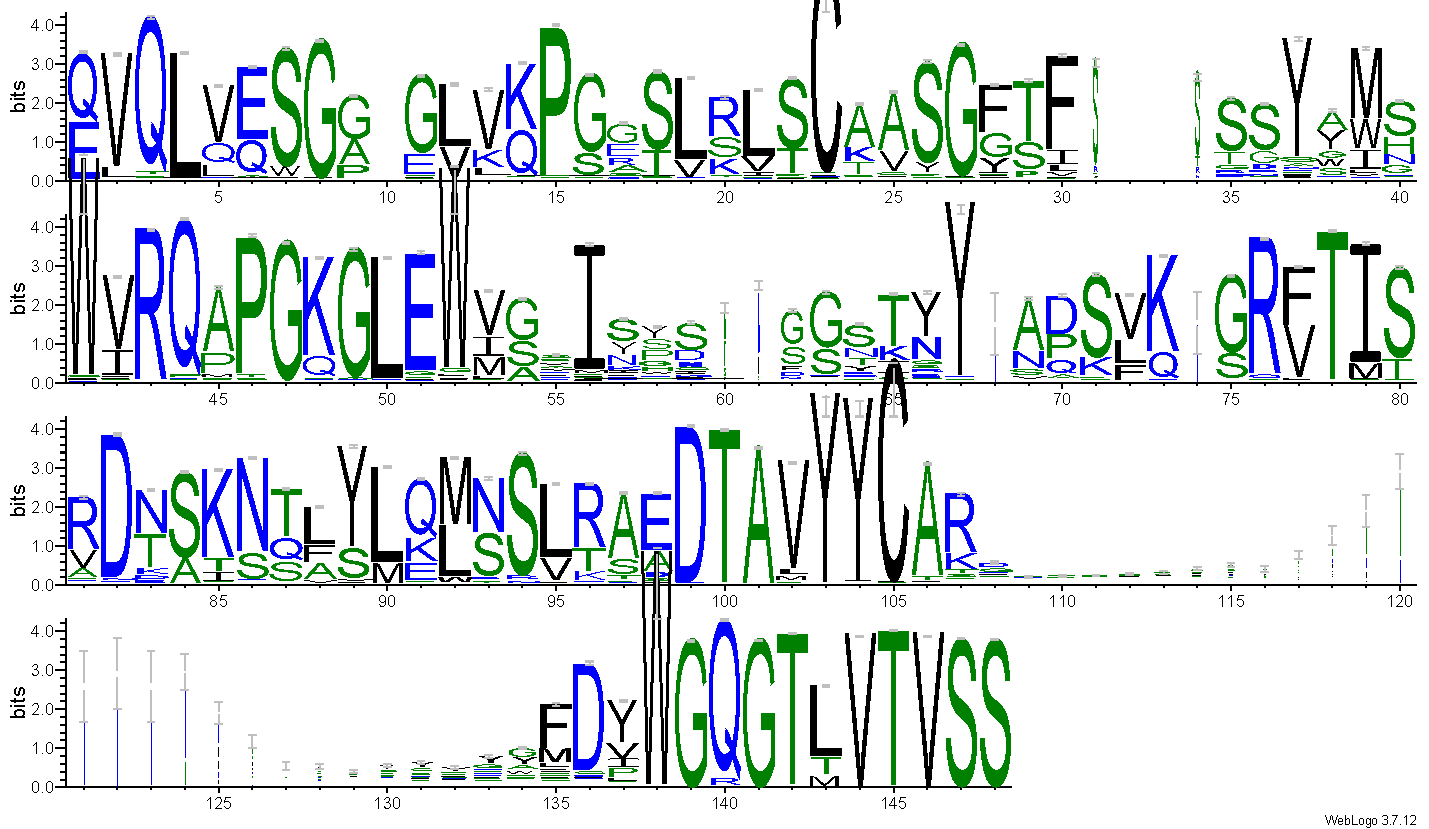
\includegraphics[width=0.9\linewidth, height=6cm]{images/human_hmm_align_logo.pdf} 
		\caption{Human}
		%\label{fig:hhmmlogo}
	\end{subfigure}
	\begin{subfigure}{0.5\textwidth}
		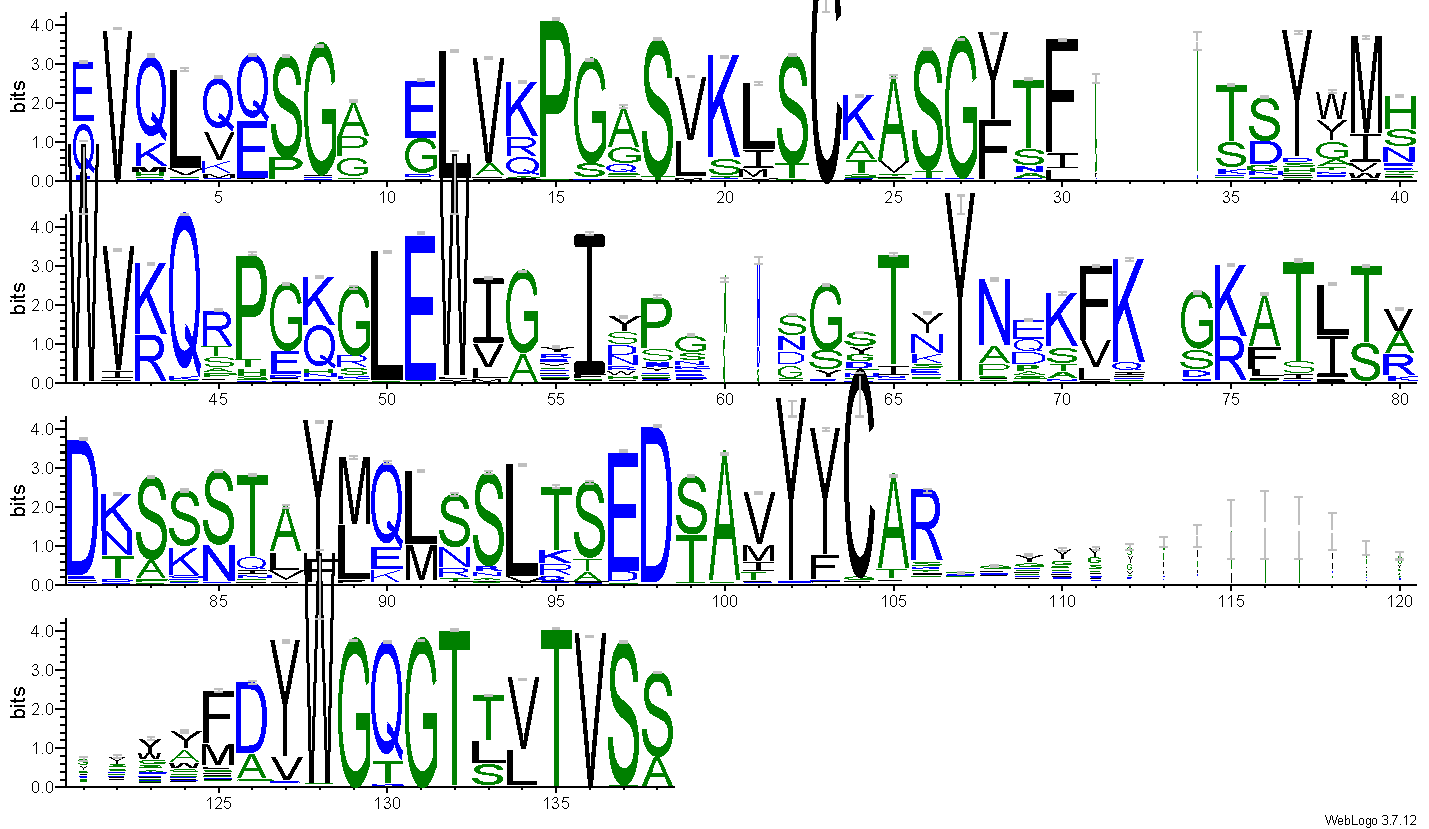
\includegraphics[width=0.9\linewidth, height=6cm]{images/mouse_hmm_align_logo.pdf}
		\caption{Mouse}
		%\label{fig:mhmmlogo}
	\end{subfigure}
	
	\caption{\small Sequence logos obtained from the alignments extracted from the antibody numbering. Human CDRs span the following positions in the plot: 26-37, 55-64, 105-136. Mouse CDRs: 26-37, 55-64, 104-126. Positions without letter are occupied mostly by gaps across the set of sequences.}
	\label{fig:image2}
\end{figure}

The lengths of the sequence logos obtained with the first Multiple Sequence Alignment are greater than those obtained through HMM and antibody numbering with IMGT. That is because \verb|anarci| aligns each sequence to a set of Hidden Markov Models (HMMs) using HMMER3. Each HMM describes the putative germ-line sequences for a domain type (VH, Vk or Vj, Va or Vb) of a particular species. The most significant alignment classifies the domain type and the alignment is then translated into a chosen numbering scheme (IMGT in our case). In other words, the second method is imposing some preconceived assumptions, while the first method is not, so the length is left free to vary more.

Moreover, thanks to the IMGT numbering, we were able to identify the domain of our sequences: it is the variable part of the heavy chain of the antibody (VH).

Another advantage of using \verb|anarci| is that the CDRs are much easier to identify because their position in the sequence can simply be retrieved from the numbering. In fact, all the sequences in the alignment have the same length; this is achieve in ANARCI by adding gaps into CDRs to compensate for the variability in length from CDRs of different antibodies. Thus, the positions in the alignment (and in the plot) does not correspond to positions in the numbering, since the numbering makes use of a convoluted notation for CDRs of different length (i.e. 111A, 111B, etc).



\section{Antibody humanization}


\subsection{Humanization tool in Python}

We developed in Python the tool that outputs whether the input sequence has higher identity to mice or human sequences and finds heavy chain sequences of therapeutic antibodies (Muromonab, Bevacizumab, Caplacizumab). The code can be found in Appendix \ref{appendix:code} and on GitHub. We used an algorithm performing local alignment which finds the subsequences that align the best. Local alignment (\verb|pairwise2.align.localxx(seq1,seq2)|) is used as it is more suitable for more divergent sequences or distantly related sequences. We set the match parameter to  \textit{x}, so identical characters have a score of \textit{1} otherwise the score is \textit{0}. The chosen gap penalty parameter is also \textit{x}, meaning there are no gap penalties.




\subsection{Identifying divergent positions}

A more efficient way to aid the humanization effort would be to spot positions in the query sequence that do not align well to human sequences and suggest them as a potential target for engineering. 

To do so, the numbering obtained with ANARCI was used, since it produces gapped sequences of the same length in which CDRs and FRs are aligned according to the IMGT scheme, thus allowing position-wise residue comparison between sequences. 

The query sequences (Muromonab, Bevacizumab, Caplacizumab) and the dataset of human sequences were concatenated in a single FASTA file that was given as input to ANARCI. The alignment was then extracted in the same way as done in the previous section, and two FASTA files were produced, one with the query sequences and one with the sequences from the dataset.

Since all the sequences have the same length, it is possible to compare position by position the residues in the query sequences with the ones in the dataset sequences. Thus, it is possible to define a measure that indicates how much each residue in the query sequence is conserved across the human sequences in order to identify regions that do not align well, which might be potential target for engineering. The position-wise frequency of each residue across the human dataset was chosen as such measure. 

In order to quickly compute the frequencies for each query sequence, a Position Frequency Matrix was computed from the dataset of human sequences; gap frequency was also included. During the computation of the frequencies, the positions in the query corresponding to a gap (-) were discarded (Figure \ref{fig:ab_similarity_plot}). The frequency was obtained dividing the counts by the number of sequences in the dataset. The frequency of gaps was plotted in order to provide a visual intuition about regions in which a low frequency in the query sequences is due to a large amount of gap in specific positions in the dataset sequences; that scenario is especially true deeply into CDRs regions, which were highlighted in yellow.



\begin{figure}[h]
    \centering
    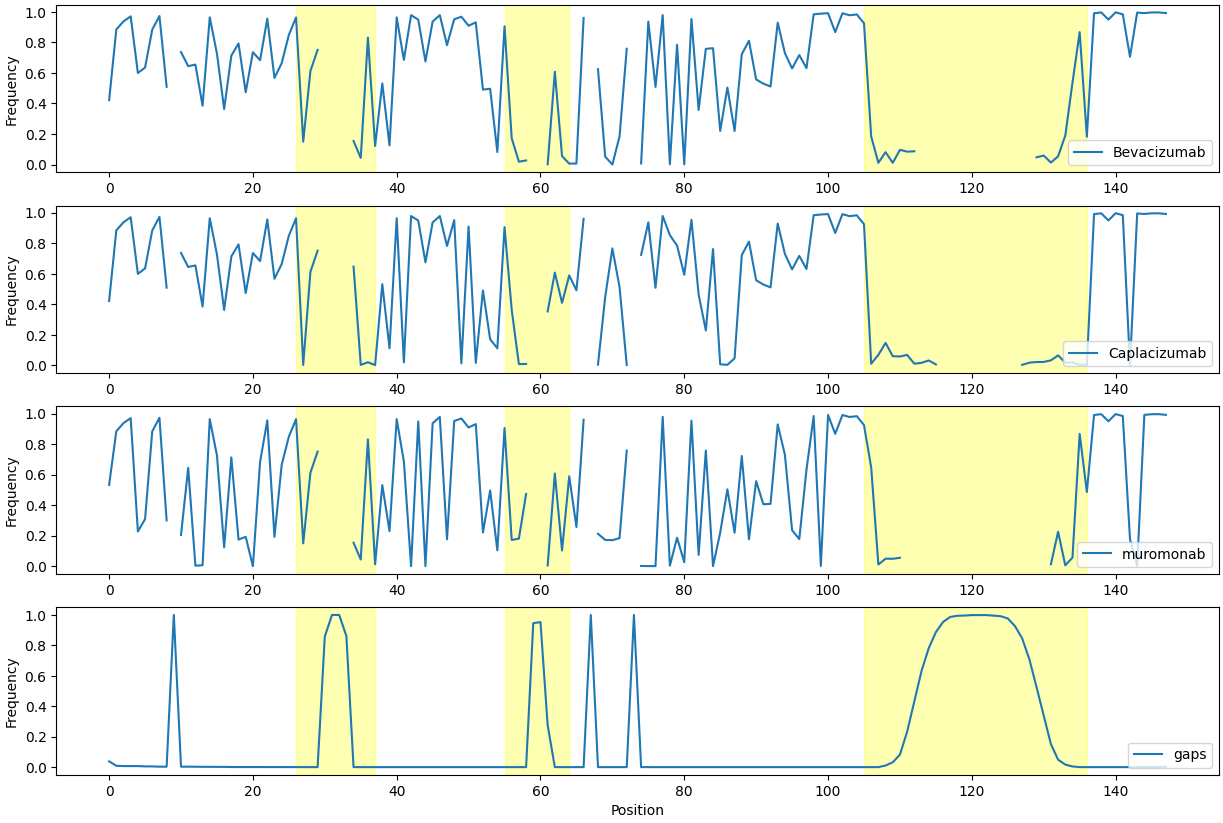
\includegraphics[width=0.87\textwidth]{images/antibody_similarity.png}
    \caption{\small Frequency of each residue found in the query sequence across the dataset of human sequences. Position covering CDRs are highlighted in yellow. The position-wise frequency of gaps in the dataset is also plotted to highlight regions in which a low frequency in the query sequences is due to a large amount of gaps in that position in the alignment.}
    \label{fig:ab_similarity_plot}
\end{figure}



As expected, the frequency suddenly drops in CDRs, while is higher in framework regions. Moreover, it is possible to spot a similarity between Bevacizumab, Caplacizumab and Muromomab in terms of the frequencies of some residues in the frameworks. This is in accordance with the fact that residues in frameworks are generally more conserved as their functions is more structural, whereas residues in the CDRs are much less conserved since they confer affinity and specificity to a given antibody. For this reason, in theory, only positions in the framework regions can be targets for engineering, since modifying the CDRs would cause the antibody to lose its function.

\subsection{Quantification of antibody nativeness using LSTM network}

A more advanced way of quantifying the nativeness of a given sequence makes use of a Long Short-Term Memory (LSTM) network published in \cite{LSTM}. The underlying assumption is that, given an input sequence, a well-trained model should be able to predict any residue by learning information from its neighbors. The output of the model is the averaged sum of negative logarithms of all conditional probabilities; so lower scores indicate a higher degree of nativeness. We trained the model on the dataset of human sequences, setting the embedding layer dimension to 128 and the hidden layer dimension to 128; other (self-explanatory) parameters we used were \verb|gapped=True| and \verb|fixed_len=True|. We plotted the frequencies of scores obtained after evaluating 20\% of the total number of human and mouse sequences [Figure \ref{fig:lstm_scores}]. As expected, human sequences score shows a peak on a lower LSTM score compared to the mouse sequences score. Also, the three therapeutic antibodies scored accordingly (Table \ref{tab:comm_score}).

\begin{figure}[th]
    \centering
    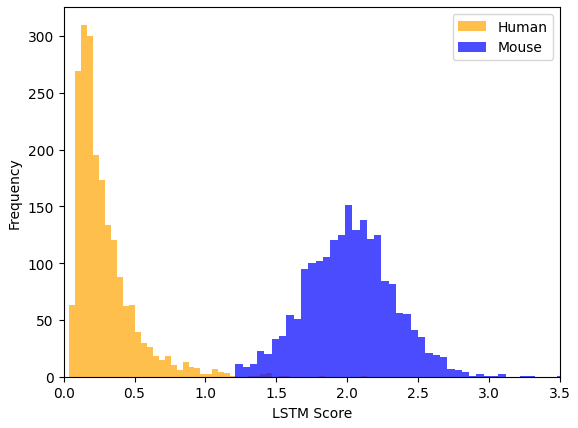
\includegraphics[width=0.7\textwidth]{images/score_plot.png}
    \caption{\small Distribution of sequence scores of human and mouse sequences obtained with the LSTM model trained on human sequences}
    \label{fig:lstm_scores}
\end{figure}

We plotted the Receiver Operating Characteristic (ROC) curve where positives correspond to human and negatives to mouse [Figure \ref{fig:roc}].
The ROC analysis shows that in classifying sequences as human-like, the model has an AUC of 0.99939 for mouse sequences.

\begin{table}[h]
    \centering
    \begin{tabular}{lcc}
        \toprule
        \textbf{Antibody} & \textbf{LSTM score}     &    \textbf{V identity}   \\
        \midrule
        Bevacizumab       &     1.50             &       0.77   \\
        Caplacizumab      &     1.72             &       0.82   \\
        Muromonab         &     1.83             &       0.72   \\
        \bottomrule
    \end{tabular}
    \caption{\small LSTM score and V gene identity of commercially available sequences. As expected, humanized antibodies (Bevacizumab and Caplacizumab) score lower than Muromomab, which is from mouse but not humanized. If plotted in the KDE plot, all the three point lie within the mouse area.}
    \label{tab:comm_score}
\end{table}


Finally, we plotted the LSTM score of human and mouses sequences versus the human germline V gene identity as a Kernel Density Estimate (KDE) plot [Figure \ref{fig:kernel}]. This identity score corresponds to the sequence identity over the v-region to the most sequence identical germline, and it was extracted from the ANARCI numbering.
As expected, we found the LSTM score to be correlated to the sequence identity of the closest human germline v-gene: the higher the identity, the lower the LSTM score. By looking at this plot, it is evident that most of the human sequences in the human dataset had a germline identity close to 1; 
\nopagebreak[1] so, the LSTM model was trained on sequences closely related to the germline sequence. 

Thus, a correlation between LSTM score and germline identity is expected a priori, since sequences with lower germline identity are expected to score higher in the evaluation simply because they are less prevalent in the training dataset. However, this correlation was maintained in mouse sequences as well, pointing to the fact that the LSTM model is able to model the sequences in a biologically relevant way.
Finally, our results were in line with the results of \cite{LSTM}.

\begin{figure}[h]
	
	\begin{subfigure}{0.5\textwidth}
		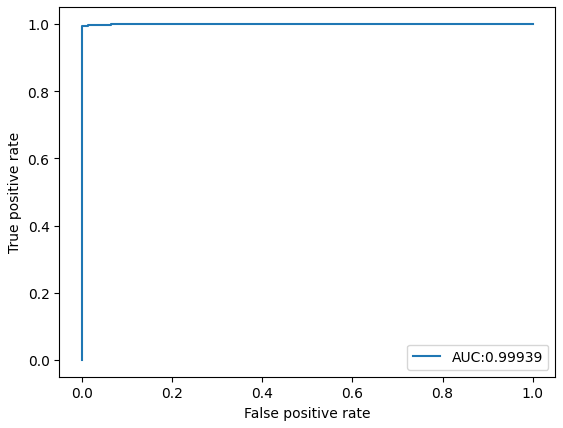
\includegraphics[width=0.9\linewidth, height=6cm]{images/ROC.png} 
		\caption{\small ROC curve}
		\label{fig:roc}
	\end{subfigure}
	\begin{subfigure}{0.5\textwidth}
		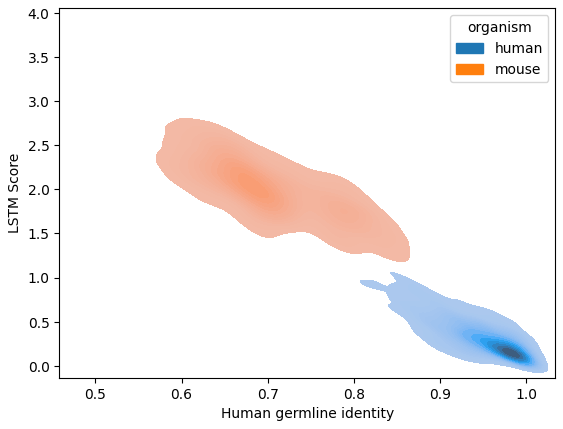
\includegraphics[width=0.9\linewidth, height=6cm]{images/score_vs_identity.png}
		\caption{\small Kernel Density Estimation}
		\label{fig:kernel}
	\end{subfigure}
	
	\caption{\small \textbf{(a)} ROC curve showing the performance of the LSTM model trained on human sequences in distinguishing human and mouse sequences. \textbf{(b)} Kernel Density Estimation plot showing the relationship between LSTM score and the identity to the V-gene computed by ANARCI.}
	\label{fig:roc_kernel}
\end{figure}



\newpage
\section{Conclusion}

In this analysis of antibody sequences, we successfully performed Multiple Sequence Alingment using different tools, we performed Antibody Numbering using ANARCI, and we explored different ways to compute the similarity between a given sequence and a dataset of human sequences to potentially aid the humanizaton effort. 




\clearpage

\appendix
\renewcommand{\thefigure}{S\arabic{figure}}
\setcounter{figure}{0}


\section{Appendix}

\subsection{Supplementary Figures}

\begin{figure}[h]
	
	\begin{subfigure}{0.5\textwidth}
		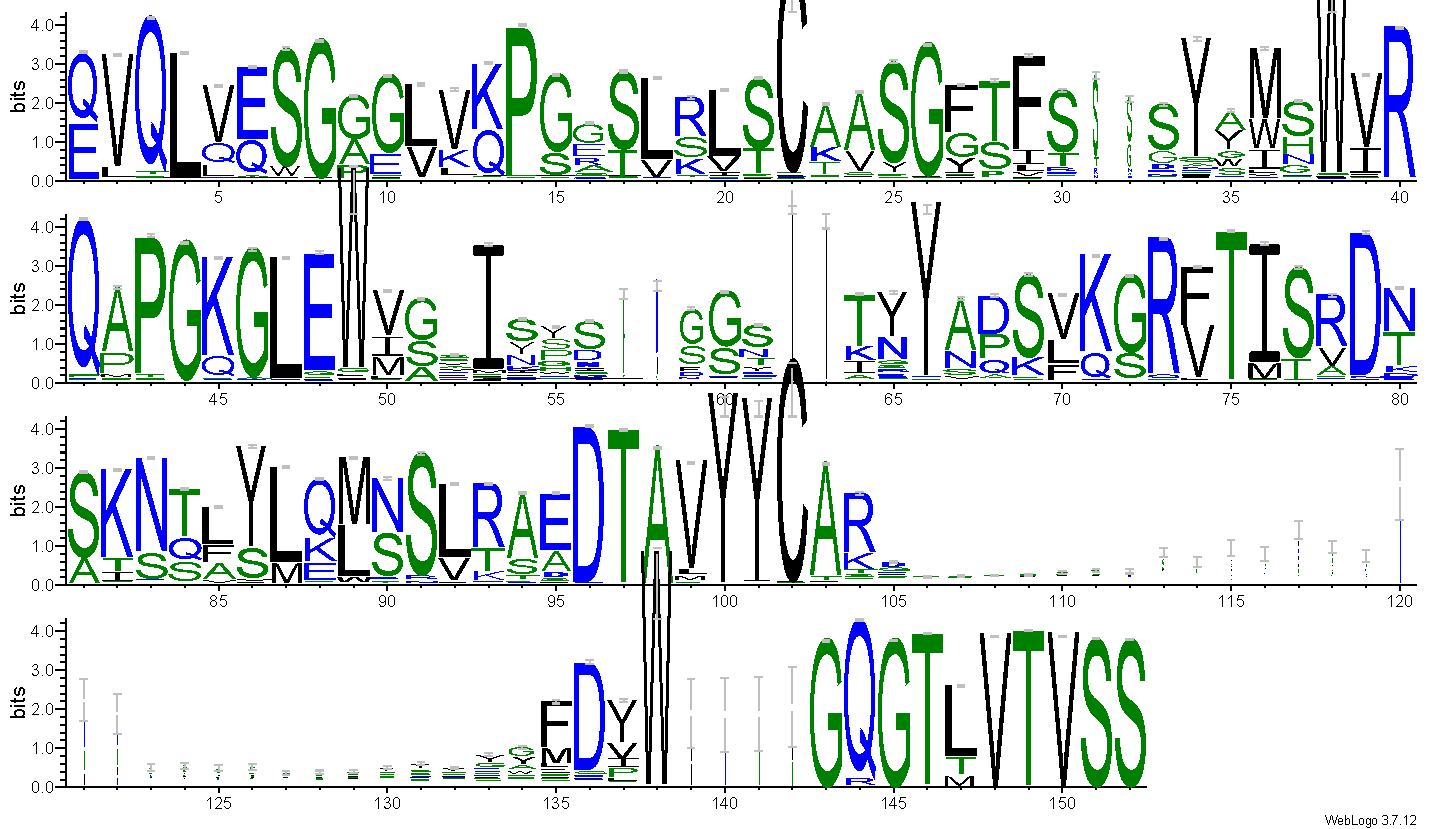
\includegraphics[width=0.9\linewidth, height=6cm]{images/human_msa_clustalO_logo.pdf} 
		\caption{Human}
		%\label{fig:hlogo}
	\end{subfigure}
	\begin{subfigure}{0.5\textwidth}
		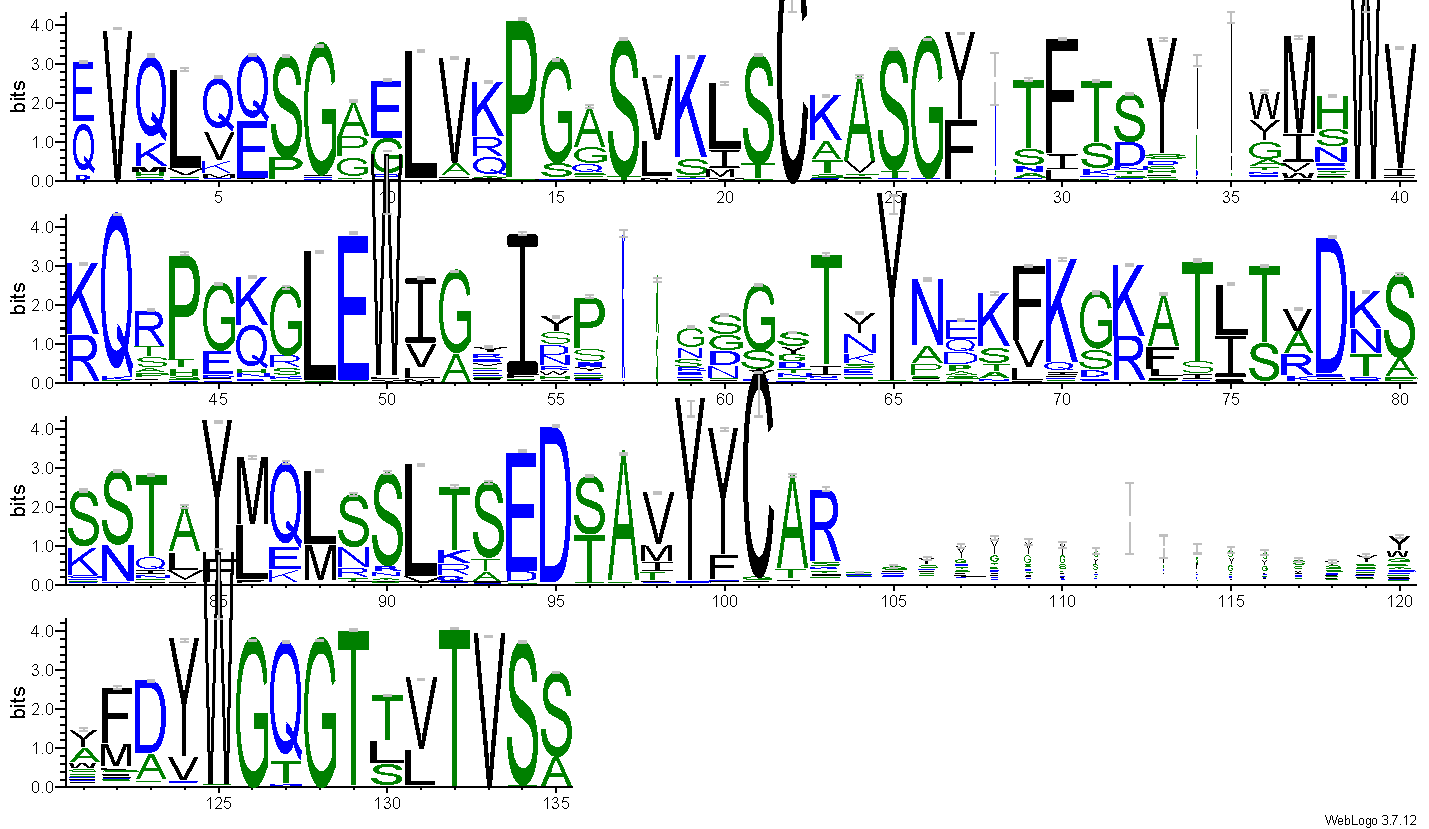
\includegraphics[width=0.9\linewidth, height=6cm]{images/mouse_msa_clustalO_logo.pdf}
		\caption{Mouse}
		%\label{fig:mlogo}
	\end{subfigure}
	
	\caption{Sequence logos for human and mouse antibody sequences aligned with Clustal Omega}
	\label{fig:clustalo_logo}
\end{figure}



\subsection{Code for humanization tool}\label{appendix:code}

\begin{minted}{python}
import Bio.SeqIO as SeqIO
from Bio import pairwise2
import os
from datetime import datetime

# get the directories
# used files have to be stored in same directory as the code
cwd = os.getcwd()
humDir = os.path.join(cwd,"human.fa")
mouseDir = os.path.join(cwd, "mouse.fa")
muromonab = os.path.join(cwd, "muromonab.FASTA")
bevacizumab = os.path.join(cwd, "bevacizumab.FASTA")
caplacizumab = os.path.join(cwd, "caplacizumab.FASTA")

# get muromonab sequence
muromonab = SeqIO.to_dict(SeqIO.parse(muromonab, "FASTA"))
muromonab = list(muromonab.values())
muromonab = muromonab[0].seq

# get bevacizumab sequence
bevacizumab = SeqIO.to_dict(SeqIO.parse(bevacizumab, "FASTA"))
bevacizumab = list(bevacizumab.values())
bevacizumab = bevacizumab[0].seq

# get caplacizumab sequence
caplacizumab = SeqIO.to_dict(SeqIO.parse(caplacizumab, "FASTA"))
caplacizumab = list(caplacizumab.values())
caplacizumab = caplacizumab[0].seq


# local alignment of given sequence with all sequences given sequences of humans and mice
# use global alignment if sequences have roughly same length else use local
def alignment(seq,humDir,mouseDir):
    print(datetime.now())
    
    # get human and mouse dicts
    humDict = SeqIO.to_dict(SeqIO.parse(humDir, "FASTA"))
    mouseDict = SeqIO.to_dict(SeqIO.parse(mouseDir, "FASTA")) 
    
    # get sequences
    humSequences = [s.seq for s in humDict.values()]
    mouseSequences = [s.seq for s in mouseDict.values()]
    
    # start alignment for all given human sequences
    print('starting pairwise alignment human dataset\n')    
    humAlignments = [pairwise2.align.localxx(seq,humS) for humS in humSequences]
    print("done pairwise alignment human dataset\n")  
    print(datetime.now())
    
    # start alignment for all given mouse sequences
    print('starting pairwise alignment mouse dataset\n')
    mouseAlignments = [pairwise2.align.localxx(seq,mouseS) for mouseS in mouseSequences]
    print("done pairwise alignment mouse dataset\n")    
    print(datetime.now())
         
    return humAlignments, mouseAlignments

# find the highest score of all possible alignments
def get_highest_score(humAlignments,mouseAlignments):

    hMax = 0
    mMax = 0
      
    # find highest score of human alignments and highest score of mouse alignments
    for hA,mA in zip(humAlignments,mouseAlignments):
        for align in hA:
            if align.score > hMax: 
                hMax = align.score
                hSeq = align.seqB
        for align in mA:
            if align.score > mMax:
                mMax = align.score
                mSeq = align.seqB
    
    # compare human and mouse highscore and return highest
    if hMax > mMax:
        return {'dataset': 'human', 'seq': hSeq, 'score': hMax}
    return {'dataset': 'mouse', 'seq': mSeq, 'score': mMax}        


hMuromonabSeq, mMuromonabSeq = alignment(muromonab, humDir, mouseDir)
highMuromonabSeq = get_highest_score(hMuromonabSeq, mMuromonabSeq)
print("highest score for alignment with muromonab: "+ str(highMuromonabSeq))

hBevacizumabSeq, mBevacizumabSeq = alignment(bevacizumab, humDir, mouseDir)
highBevacizumabSeq = get_highest_score(hBevacizumabSeq, mBevacizumabSeq)
print("highest score for alignment with bevacizumab: " + str(highBevacizumabSeq))

hCaplacizumabSeq, mCaplacizumabSeq = alignment(caplacizumab, humDir, mouseDir)
highCaplacizumabSeq = get_highest_score(hCaplacizumabSeq, mCaplacizumabSeq)
print("highest score for alignment with caplacizumab: " + str(highCaplacizumabSeq))

\end{minted}


\clearpage


\printbibliography


\end{document}